\documentclass{beamer}

\usepackage{booktabs}
\usepackage{graphicx}
\usepackage{verbatim}
\usepackage{tikz}
\usetikzlibrary{shapes, arrows}

\setbeamertemplate{navigation symbols}{}

\title{Pythons and Ladders}
\author{James Campbell}
\institute[Cardiff University]
  {
  Department of Mathematics\\
  Cardiff University
  }
\date{Django Conference, 2014}

\begin{document}

\begin{frame}
  \titlepage
\end{frame}

\begin{frame}{The Game}
    \begin{center}
      \includegraphics[scale=2.2]{images/SALboard}
    \end{center}
\end{frame}

\begin{frame}{Modelling the Game}
  \begin{itemize}
    \itemsep2em
    \item Absorbing Markov Chain

    \item Transition Matrix
  \end{itemize}
\end{frame}

\frame{\frametitle{The Approach}
\begin{center}
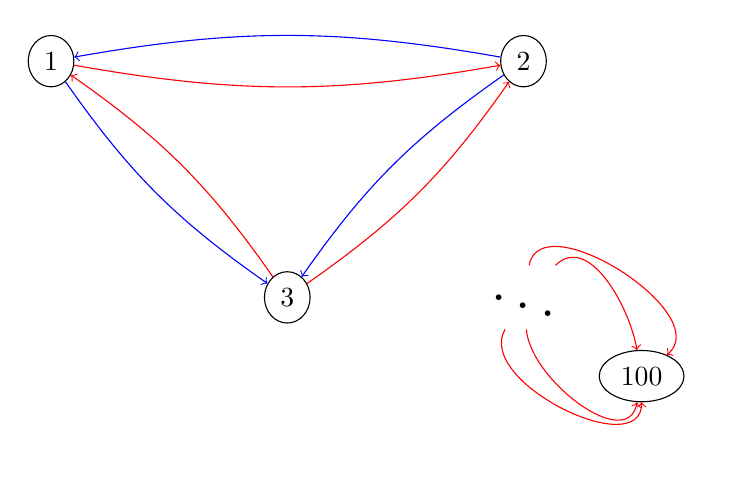
\begin{tikzpicture}
\node (A) at (0,0) [draw, ellipse] {$1$};
\node (B) at (6,0) [draw, ellipse] {$2$};
\node (C) at (3,-3) [draw, ellipse] {$3$};

\pause
\draw (A) edge[out=-10, in= -170, ->, red] (B);
\draw (B) edge[in=10, out= 170, ->, blue] (A);

\draw (C) edge[out=35, in= -125, ->, red] (B);
\draw (B) edge[in=55, out= -145, ->, blue] (C);

\draw (C) edge[out=125, in= -35, ->, red] (A);
\draw (A) edge[in=145, out= -55, ->, blue] (C);

\node (otherstates) at (6,-3) {\Huge{$\ddots$}};

\node (absorption) at (7.5,-4) [draw, ellipse] {$100$};

\draw (otherstates) edge[out=45, in=100, ->, red] (absorption);
\draw (otherstates) edge[out=-85, in=-100, ->, red] (absorption);
\draw (otherstates) edge[out=-120, in=-90, ->, red] (absorption);
\draw (otherstates) edge[out=80, in=40, ->, red] (absorption);


\end{tikzpicture}
\end{center}
}

\begin{frame}[fragile]{Some Code}
  \begin{verbatim}
a = matrix(QQ, 101)

SaLdic = {29: 7,
          71: 53,
          93: 1,
          97: 61,
          14: 64,
          30: 49,
          39: 60,
          67: 96,
          }
  \end{verbatim}
\end{frame}

\begin{frame}[fragile]{More Code}
  \begin{verbatim}
def rolldie(N):
    for i in range(1,7):
        if N + i <= 100:
            a[N, N + i] = 1/6
        else:
            a[N, N] += 1/6
  \end{verbatim}
\end{frame}

\begin{frame}[fragile]{Still More Code}
  \begin{verbatim}
for k in range(100):
    if k not in SaLdic:
        rolldie(k)

for p, q in SaLdic.iteritems():
    a[p, q] = 1
  \end{verbatim}
\end{frame}

\begin{frame}{Transition Matrix}
    \begin{center}
      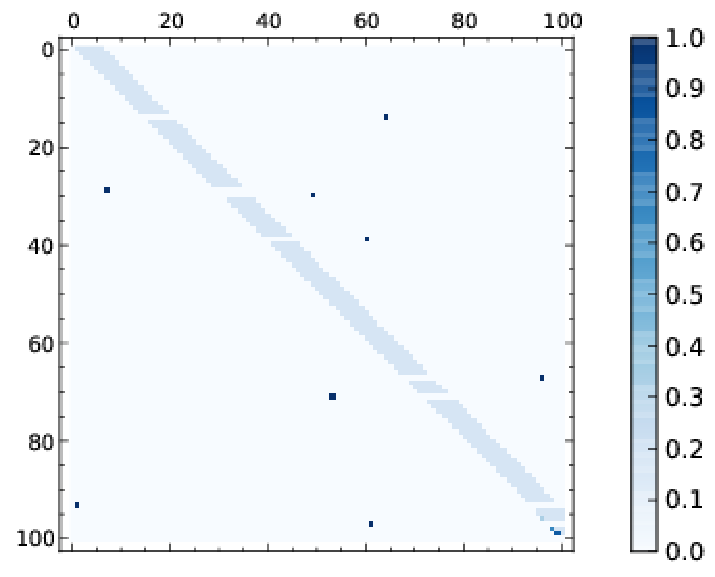
\includegraphics[scale=0.8]{images/matplot}
    \end{center}
\end{frame}

\begin{frame}{Results - Where will you be?}
  \begin{columns}
    \column{.5\textwidth}
      \begin{center}
      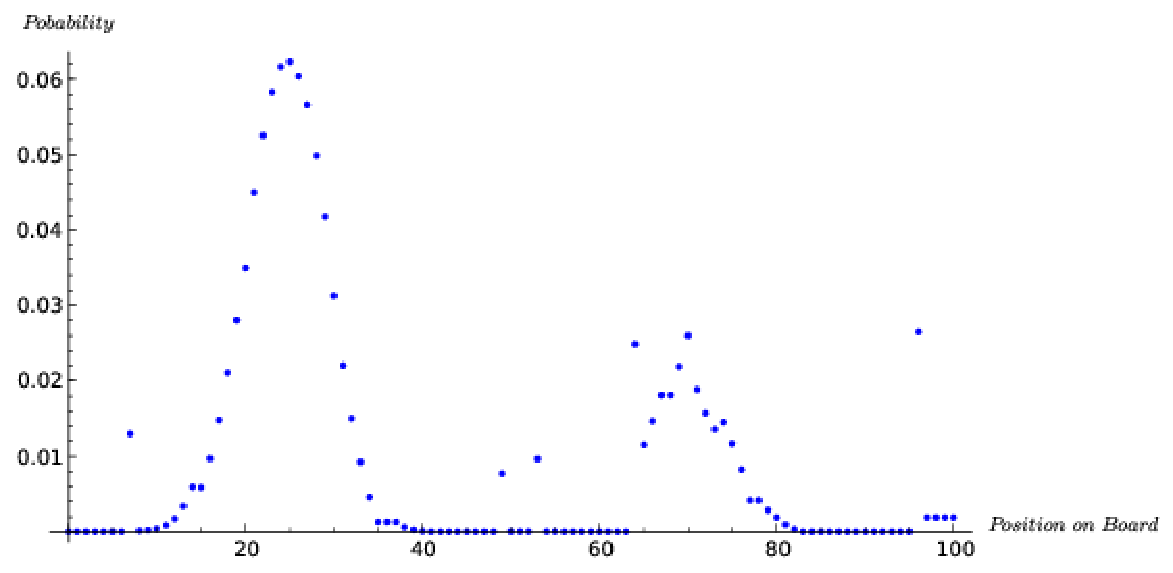
\includegraphics[width=\linewidth]{images/7plot}\\
      7 rolls
      \end{center}
    \column{.5\textwidth}
      \begin{center}
      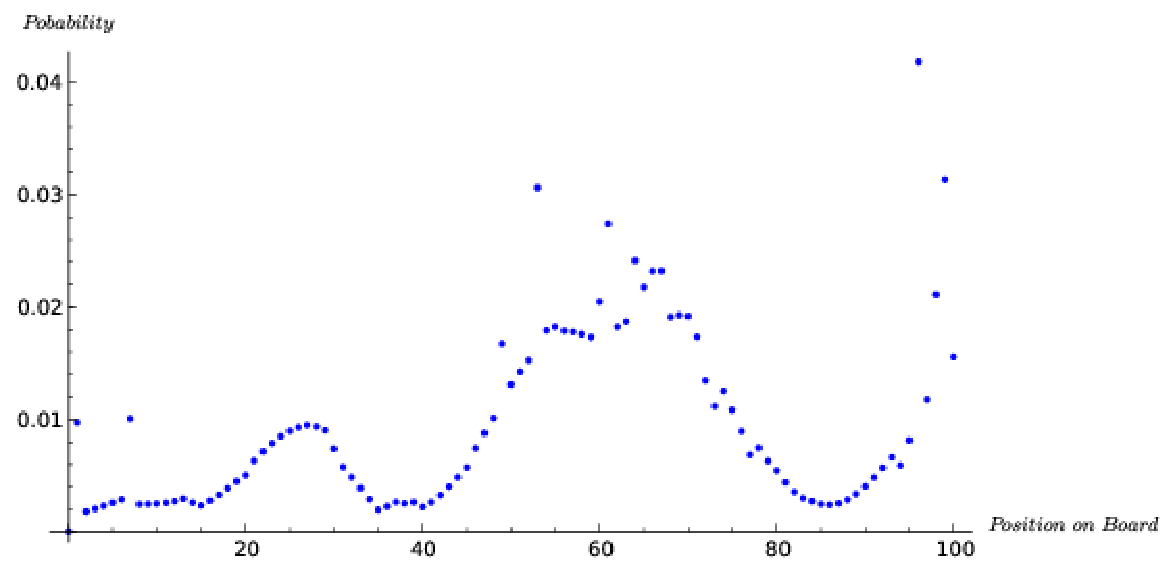
\includegraphics[width=\linewidth]{images/15plot}\\
      15 rolls
      \end{center}
  \end{columns}
\end{frame}

\begin{frame}{Results - How long is a game likely to last?}
  \begin{columns}
    \column{.5\textwidth}
      \begin{center}
      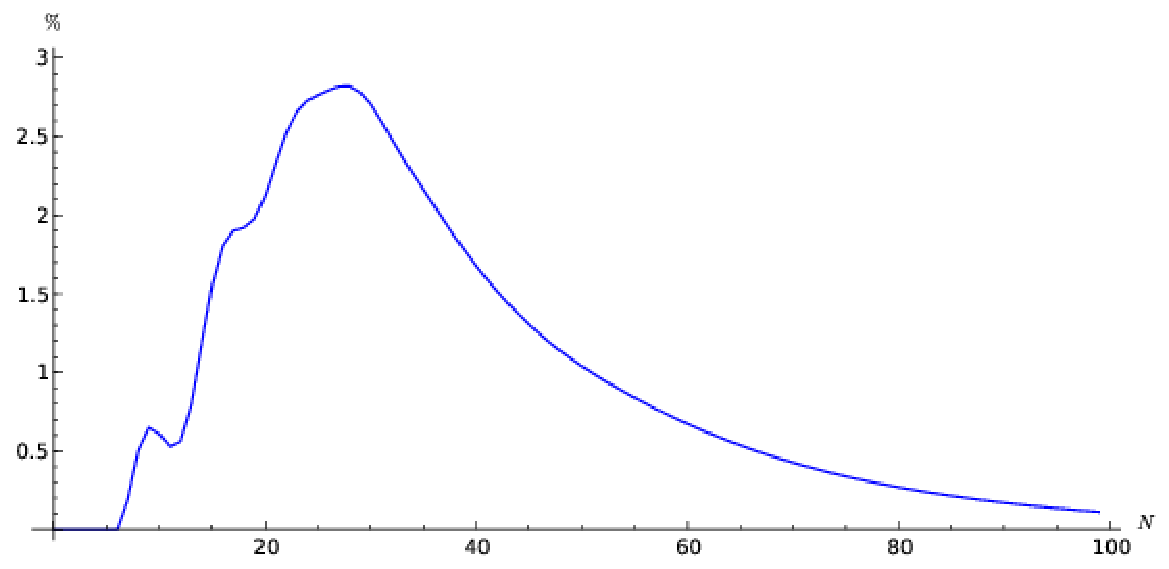
\includegraphics[width=\linewidth]{images/turns}\\
      The Percentage of games that end ON turn $N$.
      \end{center}
    \column{.5\textwidth}
      \begin{center}
      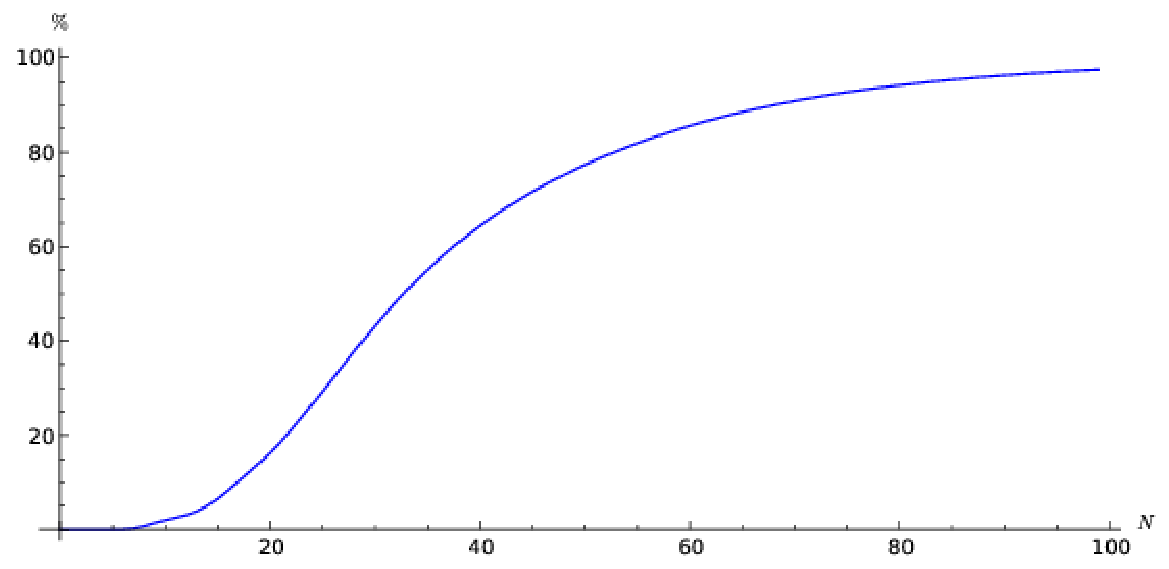
\includegraphics[width=\linewidth]{images/sumturns}\\
      The Percentage of games that end BY turn $N$.
      \end{center}
  \end{columns}
\end{frame}

\begin{frame}{Contact Me}
  \begin{itemize}
    \itemsep2em
    \item Email: \href{mailto:campbellj11@cardiff.ac.uk}{campbellj11@cardiff.ac.uk}

    \item GitHub: \href{https://github.com/theref}{www.github.com/theref}

    \item LinkedIn
  \end{itemize}
\end{frame}

\end{document}
